\documentclass[a4paper,11.5pt,table]{article}
\usepackage[textwidth=170mm, textheight=230mm, inner=20mm, top=20mm, bottom=30mm]{geometry}
\usepackage[normalem]{ulem}
\usepackage[utf8]{inputenc}
\usepackage[T1]{fontenc}
\PassOptionsToPackage{defaults=hu-min}{magyar.ldf}
\usepackage[magyar]{babel}
\usepackage{amsmath, amsthm,amssymb, paralist, tikz, multirow, float}
\usetikzlibrary{arrows, positioning}

\usepackage{listings}
\lstdefinestyle{customc}{
	belowcaptionskip=1\baselineskip,
	breaklines=true,
	frame=L,
	language=C++,
	showstringspaces=false,
	basicstyle=\ttfamily,
	%identifierstyle=\color{blue},
	keywordstyle=\bfseries\color{green!40!black},
	stringstyle=\color{orange},
	emph = {std, A, B, BDIT, Base, BaseOne, BaseTwo, C, CharT, Circle, Compr, ConstIterator, Cont, D, Deltoid, Derived, Derived2, DerivedLast, DerivedOne, DerivedTwo, Fact, Fiu, Foo, Greater, Hallgato, IT, InputIt, Iterator, Kor, Lany, Less, LessByX, LinAlgVector, List, Matrix, Negyszog, Negyzet, RAIT, Rombusz, S, Sielo, Sikidom, StringLength, T, T1, T2, Templ, U, Val, X, Y, Z, bad_cast, bidirectional_iterator_tag, const_iterator, deque, forward_iterator_tag, input_iterator_tag, iostream, istream, iterator, iterator_category, line_editor, list, map, multimap, multiset, ostream, pair, random_access_iterator_tag, set, string, strlen, strlenWrong, value_type, vector}, 
	emphstyle = \color{blue},
	tabsize = 4
}

\lstdefinestyle{customasm}{
	belowcaptionskip=1\baselineskip,
	frame=L,
	language=[x86masm]Assembler,
	basicstyle=\ttfamily,
	commentstyle=\itshape\color{purple!40!black},
}

\lstset{
	escapechar=@,
	style=customc,
	literate =  {á}{{\'a}}1 {é}{{\'e}}1 {í}{{\'i}}1 {ó}{{\'o}}1 {ú}{{\'u}}1
	{Á}{{\'A}}1 {É}{{\'E}}1 {Í}{{\'I}}1 {Ó}{{\'O}}1 {Ú}{{\'U}}1
	{ö}{{\"o}}1 {ü}{{\"u}}1 {Ö}{{\"O}}1 {Ü}{{\"U}}1
	{ű}{{\H{u}}}1 {Ű}{{\H{U}}}1 {ő}{{\H{o}}}1 {Ő}{{\H{O}}}1
	{€}{{\euro}}1 {£}{{\pounds}}1	
}

\lstset{escapechar=@,style=customc}

\usepackage{hyperref}

\begin{document}
	%%%%%%%%%%%RÖVIDÍTÉSEK%%%%%%%%%%
	\setlength\parindent{0pt}
	\def\<{<\hspace{0mm}<}
	
	\theoremstyle{definition}
	\newtheorem{note}{Megjegyzés}[subsection]
	%%%%%%%%%%%%%%%%%%%%%%%%%%%%%%%%%%%%%%%%%%%%%%%%%%%%%%%%%%%%%%%%%%%%%
	
	\begin{center}
		{\LARGE\textbf{C++}}
		
		{\Large Gyakorlat jegyzet}
		
		4. óra.
	\end{center}
	A jegyzetet \textsc{Umann} Kristóf készítette \textsc{Horváth} Gábor gyakorlatán. (\today)
	
	\section{Literálok}
	\subsection{Karakterláncok}
	Mi lesz a \texttt{"Hello"} karakterlánc literál típusa?
	\smallskip
	
	Egy konstans karakterekből álló 6 méretű tömb (\texttt{const char[6]}). Azért 6 elemű, mert a karakterlánc literál végén el van tárolva a végét jelző \texttt{\textbackslash 0} karaktert.
	
	\begin{center}
		\setlength{\extrarowheight}{2pt}
		\begin{tabular}{|c|c|c|c|c|c|}
			\hline
			H&E&L&L&O&$\backslash$0\\
			\hline
		\end{tabular}
	\end{center}
	
	\vspace{-4mm}
	\begin{lstlisting}
int main()
{
	char* hello= "Hello";
	hello[1] = 'o';
}
	\end{lstlisting}
	A fenti kódban megsértettük a konstans korrektséget, hisz egy nem konstansra mutató pointerrel mutatuk egy konstans karakterlánc literál első elemére. Ennek ellenére, a fenti kód lefordul. Ennek az az oka, hogy az eredeti C-ben nem volt const kulcsszó, a kompatibilitás végett ezért C++ban lehet konstans karakterlánc literál elemire nem konstansra mutató pointerrel mutatni.
	\begin{note}
		Ezt a fajta kompatibilitás miatt meghagyott viselkedést kerülni kell. Lefordul, de kapunk rá warningot.
	\end{note}
	Ha módosítani próbáljuk a karakterlánc literál értékét, az nem definiált viselkedéshez vezet. 
	%TODO Sajnos ebből nem tudtam jobb leírást kipofozni tudáshiány végett.
	
	Futtatáskor linuxon futási idejű hibát kapunk, méghozzá szegmentálási hibát. Ennek az az oka, hogy a konstansok értékei readonly memóriában vannak tárolva, aminek a módosítását nem engedi az operációs rendszer.
  \medskip
	
	Ez jól rámutat arra, hogy miért is nem jó az, ha a fenti konverziót megengedjük.
	\subsection{Szám literálok}
	Függően attól, hogy egy szám literált hogyan írunk C++ban, mást jelenthet:
	\begin{center}
		\setlength{\extrarowheight}{2pt}
		\begin{tabular}{|c|l|}
			\hline
			\texttt{5}						&\texttt{int}\\
			\hline
			\texttt{5.}						&\texttt{double}\\
			\hline
			\texttt{5.f}					&\texttt{float}\\
			\hline
			\texttt{5e-4}					&\texttt{double}, értéke 0.0005\\
			\hline
			\texttt{5e-4f}					&\texttt{float}\\
			\hline
			\multirow{2}{*}{\texttt{0xFF}}	&{16-os számrendszerben}\\
											& ábrázolt \texttt{int}\\
			\hline
			\multirow{2}{*}{\texttt{012}}	&{8-as számrendszerben}\\
											&ábrázolt \texttt{int}\\
			\hline
			\texttt{5l}						&\texttt{long int}\\
			\hline
			\texttt{5u}						&\texttt{unsigned int}\\
			\hline
			\texttt{5ul}					&\texttt{unsigned long int}\\
			\hline
		\end{tabular}
	\end{center}
	Létezik C++ban \texttt{signed} kulcsszó, mely a char miatt lett bevezetve. A char is egész számokat tartalmaz, de az implementáció függő, hogy a \texttt{char} singed vagy unsigned értéket tartalmaz-e. 
	
	Természetesen leggyakrabban egész számoknál szoktuk használni. Alapértelmezetten minden \texttt{int} egy \texttt{signed int}, amennyiben egy előjel nélküli egész számra van szükségünk, \texttt{unsigned int}-et vagy röviden \texttt{unsigned}-t kell írnunk. Megállapítható, hogy az \texttt{unsigned} típusok ugyanannyi számjegyet tudnak tárolni, ám értékben kétszer akkorát. 
	
	Míg a túlcsordulás \texttt{signed} típusoknál nem definiált, addig \texttt{unsigned} típusoknál az, a maximális érték (mely implementációfüggő) utáni inkrementális 0-ra állítja a változót. Értelemszerűen, ez a determinisztikus viselkedés futási idejű költséggel jár.
	%NOTE https://www.youtube.com/watch?v=yG1OZ69H_-o - CppCon 2016: Chandler Carruth “Garbage In, Garbage Out: Arguing about Undefined Behavior..."
	
	\medskip
	Mint tudjuk, a nem egész számoknál a törtrészt magyarban vesszővel, C++ban ponttal választjuk el. Azonban mégis, az alábbi kód helyesen lefordul:
	\begin{lstlisting}
int pi = 3,14;
	\end{lstlisting}
	Ennek oka az, hogy a vessző operátor egy szekvenciapont is, így a fordító az egyenlőség bal oldalát amikor kiértékeli, először rendre kiértékeli a 3 számliterált, eldobja, utána kiértékeli a 14-et, és értékül adja \texttt{pi}-nek. Ez azt jelenti, hogy az ilyen jellegű hibát nem olyan könnyű megfogni, mint elsőre gondolnánk.
	
	\smallskip
	A lebegőpontos számok másik veszélye, az összehasonlítás. Jusson eszünkbe, ami Numerikus Módszereken hangzik el: minden lebegőpontos szám tartalmazhat egy kis pontatlanságot.
	\begin{lstlisting}
for (double d = 0; d != 1; d += 0.1)
{
	std::cout << d << ' ';
}
	\end{lstlisting}
	Itt bár azt várnánk, hogy a kimenet \texttt{0 0.1 0.2 ... 1.0} legyen, legnagyobb valószínűséggel végtelen ciklusba futunk. Ez amiatt van, hogy a 0.1 (várhatóan) tartalmaz egy kis pontatlanságot, és így hiába írja ki  a programunk hogy \texttt{d} értéke 1, az várhatóan csak nagyon közel lesz hozzá.
	\begin{note}
		Viszonylag kevés esetben éri meg \texttt{float}-ot használni \texttt{double} helyett. Modern CPU-k ugyanolyan hatékonyan dolgoznak mind a kettővel, így érdemesebb a pontosabbat választani. (Ha magát a GPU-t programozzuk, az lehet egy kivétel.)
	\end{note}
	\begin{note}
		Érdemes mindig \texttt{int}et használnunk, ha nincs jó okunk arra, hogy mást használjunk. Az \texttt{int}-el általában a leghatékonyabb a processzor.
	\end{note}
	\subsection{Aritmetikai konverziók}
	Meglepő módon, két \texttt{int} szám hányadosa C++ban nem lebegőpontos típussal fog rendelkezni, hanem szintúgy \texttt{int}-el. A primitív típusok között szigorú konverziós szabály van. Amennyiben például azt szeretnénk, hogy a 10/4 osztás végeredménye ne egész legyen, akkor az \texttt{/} operátor legalább egyik operandusának lebegőpontosnak kell lennie, pl. így: \texttt{10/4.0}
	
	Általános szabály az, hogy ha két típus eltér aritmetikai műveleteknél, akkor konvertálni kell, és mindig a kisebb méretű típust konvertáljuk a nagyobba.
	\begin{compactenum}
		\item Ha az egyik típusa \texttt{long double}, akkor a másikat is \texttt{long double}-ra konvertáljuk.
		\item Különben ha az egyik operandus \texttt{double}, akkor másik is \texttt{double} lesz.
		\item Különben, ha az egyik \texttt{float}, akkor a másik is \texttt{float} lesz.
		\item Amennyiben egyik operandus se lebegőpontos, akkor ha az egyik operandus \texttt{unsigned long}, akkor a másik is ez lesz.
		\item Ha az egyik operandus \texttt{long}, a másik pedig \texttt{unsigned int}, akkor előfordulhat az, hogy a két típus ugyanakkora tárterületen van tárolva (a primitív típusok méreteiről később lesz részletesekben szó). Ha az \texttt{int} és a \texttt{long} mérete megegyezik, akkor \texttt{unsigned
			long} lesz mindkét operandus. Különben ha a \texttt{long} nagyobb, akkor \texttt{long}-gá konvertálódik a másik.
		\item Különben ha az egyik \texttt{long}, a másik pedig NEM \texttt{unsigned int}, akkor \texttt{long}-gá konvertálódik a másik operandus.
		\item Különben, ha az egyik operandus \texttt{unsigned int}, a másik is kovnertálódik \texttt{unsigned int}-té.
		\item Különben minden \texttt{int}-té konvertálódik, ha egyik korábbi sem teljesült.
	\end{compactenum}
	\section{Struktúrák mérete}
	\subsection{Primitív típusok mérete}
	A \texttt{sizeof(char)} mindig 1-et ad vissza. A karakter mérete mindig az egység. Minden más típusra a \texttt{sizeof} függvény azt adja vissza, hogy paraméterül megadott objektum vagy típus mérete hányszorosa a \texttt{char}nak. 
	
	Attól, hogy \texttt{sizeof(char) == 1}, a \texttt{char} mérete byteokban még implementáció függő.
	
	A lebegőpontos számok mindig rendelkeznek előjellel. 
	
	\medskip
	A \texttt{char} méretén túl minden másnak a mérete implementációfüggő, bár a szabvány kimond pár relációt:
	\begin{center}
		\texttt{sizeof(X) == sizeof(signed X) == sizeof(unsigned X)}
		\smallskip
		
		\texttt{sizeof(float) $\leq$ sizeof(double) $\leq$ sizeof(long double)}
		\smallskip
		
		\texttt{sizeof(short) $\leq$ sizeof(int) $\leq$ sizeof(long)}
		\smallskip
		
		\texttt{sizeof(char) $\leq$ sizeof(bool)}
		\smallskip
	\end{center}
	\subsection{Nem primitív típusok mérete}
	Egy áltlaunk megalkotott típus mérete több szabálytól is függhet.
	\begin{lstlisting}
#include <iostream>

struct Hallgato
{
	double atlag;
	int kor;
	int magassag;
}

int main()
{
	std::cout << sizeof(double) << std::endl;
	std::cout << sizeof(int) << std::endl;
	std::cout << sizeof(Hallgato) << std::endl;
}
	\end{lstlisting}
	A gyakorlaton használt gépen a \texttt{double} mérete 8, az \texttt{int} mérete 4, \texttt{Hallgato}-é 16. Ezen azt látjuk, hogy a \texttt{Hallgato} tiszta adat.
	\begin{lstlisting}
struct Hallgato
{
	int kor;
	double atlag;
	int magassag;
}
	\end{lstlisting} 
	Miután átrendeztük a mezők sorrendjét, és újra kiírjuk a struktúra méretét, akkor a válasz 24. Ennek az oka az, hogy míg az első esetben így volt eltárolva a memóriában: (ne feledjük, ez még mindig implementációfüggő!)
	\begin{figure}[H]
		\centering
		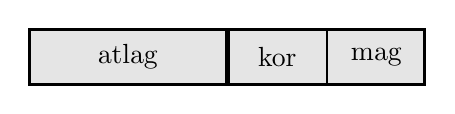
\begin{tikzpicture}
		\tikzstyle{Node} = [rectangle, minimum width=2.5cm, minimum height=7mm, text centered, draw=black, fill= gray!20, line width = 1.2pt]
		\tikzstyle{Border} = [rectangle, minimum width=2.5cm, minimum height=7mm, text centered, draw=black, line width = 1.2pt]
		\tikzstyle{HalfNode} = [rectangle, minimum width=1.25cm, minimum height=7mm, text centered, draw=black, fill= gray!20, line width = 0.2pt]
		\tikzstyle{arrow} = [thick,->,>=stealth]
		
		\node (1) [Node] {atlag};
		\node (2) [HalfNode, right = 0mm of 1] {kor};
		\node (3) [HalfNode, right = 0mm of 2] {mag};
		\node (border) [Border, right = -0.2mm of 1] {};
		
		\end{tikzpicture}
	\end{figure}
	Azaz, \texttt{atlag}, illetve \texttt{kor} és \texttt{magassag} pont efértek 1-1 gépi szóban. Viszont, ha megcseréljük a sorrendet, ez már nem lesz igaz:
	\begin{figure}[H]
		\centering
		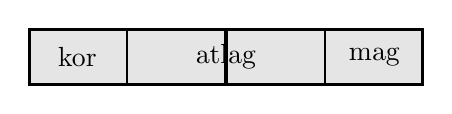
\begin{tikzpicture}
		\tikzstyle{Node} = [rectangle, minimum width=2.5cm, minimum height=7mm, text centered, draw=black, fill= gray!20]
		\tikzstyle{Border} = [rectangle, minimum width=2.5cm, minimum height=7mm, text centered, draw=black, line width = 1.2pt]
		\tikzstyle{HalfNode} = [rectangle, minimum width=1.25cm, minimum height=7mm, text centered, draw=black, fill= gray!20, line width = 0.2pt]
		\tikzstyle{arrow} = [thick,->,>=stealth]
		
		\node (1) [HalfNode] {kor};
		\node (2) [Node, right = 0mm of 1] {atlag};
		\node (3) [HalfNode, right = 0mm of 2] {mag};
		\node (border) [Border, right = -1.26cm of 1] {};
		\node (border) [Border, left = -1.26cm of 3] {};
		\end{tikzpicture}
	\end{figure}
  Itt az \texttt{atlag} két fele két különböző gépi szóba kerülne. Ez a ma használt processzorok számára nem hatékony, hiszen az átlag értékének kiolvasásához vagy módosításához két gépi szót is olvasni vagy módosítani kéne (a legtöbb processzor csak szóhatárról tud hatékonyan olvasni).
	\begin{figure}[H]
		\centering
		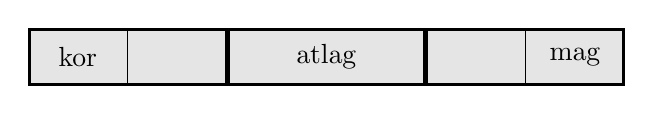
\begin{tikzpicture}
		\tikzstyle{Node} = [rectangle, minimum width=2.5cm, minimum height=7mm, text centered, draw=black, fill= gray!20, line width = 1.2pt]
		\tikzstyle{HalfNode} = [rectangle, minimum width=1.25cm, minimum height=7mm, text centered, draw=black, fill= gray!20, line width = 0.2pt]
		\tikzstyle{Border} = [rectangle, minimum width=2.5cm, minimum height=7mm, text centered, draw=black, line width = 1.2pt]
		\tikzstyle{arrow} = [thick,->,>=stealth]
		
		\node (1) [Node] {atlag};
		\node (2) [HalfNode, left = 0mm of 1] {};
		\node (3) [HalfNode, left = 0mm of 2] {kor};
		\node (4) [HalfNode, right = 0mm of 1] {};
		\node (5) [HalfNode, right = 0mm of 4] {mag};
		\node (border) [Border, right = -0.2mm of 1] {};
		\node (border) [Border, left = -0.2mm of 1] {};
		\end{tikzpicture}
	\end{figure}
	A fenti elrendezés hatékonyabb, bár 3 gépi szót használ. Ebben az esetben a fordító \textit{padding}et illeszt be a mező után. Ennek hatására hatékonyan olvasható és módosítható minden mező. Cserébe több memóriát foglal a struktúra.
	\smallskip
	
	A szabvány kimondja, hogy egy \texttt{struct} mérete az adottagok méreteinek összegénél nagyobb vagy egyenlő.
	\smallskip
	
	Az, hogy egy gépi szó mekkora, implementációfüggő.
	\bigskip
	
	Egy \texttt{struct} egyes adattagjaira a pont operátor segítségével hivatkozhatunk:
	\begin{lstlisting}
int main()
{
	//...
	Hallgato a;
	std::cout << a.kor << std::endl;
	Hallgato b = a;
	b.magassag = 3;
}
	\end{lstlisting}      
	
\end{document}
